
\begin{exercise}

 \begin{minipage}[t]{.62\linewidth}
Een massa blijft liggen op een draai\-tafel die met een hoeksnelheid van \SI{5,0}{rad/s} draait. Ze ligt op een afstand van \SI{10}{cm} van het middelpunt.
\newline
\newline
Hoe groot moet de wrijgvingsco\"effici\"ent tussen de massa en de tafel minstens zijn? Toon aan.
\end{minipage}
%\hspace{.05\linewidth}
\hfill
\begin{minipage}[t]{.33\linewidth}
	\raisebox{1ex-\height}{%
    	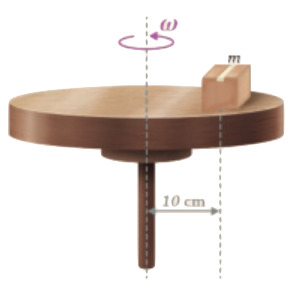
\includegraphics[width=\linewidth]{dyn/exercises/FV6p153}
  	}%
\end{minipage}

\begin{oplossing}
	De middelpuntzoekende kracht wordt door de wrijvingskracht geleverd. De maximale grootte hiervan wordt gegeven door $\mu F_n$. De hoeksnelheid die we nog net kunnen aanhouden zonder dat de massa's schuiven, vinden we met de tweede wet van Newton:
	\begin{eqnarray*}
		\vec{F}&=&m\vec{a}\\
		&\Downarrow&\\
		\mu mg&=&mr\omega^2
		%\Leftrightarrow\omega&=&\sqrt{\frac{\mu g}{r}}
	\end{eqnarray*}
	of
		\begin{eqnarray*}
\omega=\sqrt{\frac{\mu g}{r}}
	\end{eqnarray*}
Omdat de massa geen rol speelt in deze formule (voor een grotere massa is een grotere middelpuntzoekende kracht nodig maar de normaalkracht wordt evenredig groter voor grotere massa's), bepaalt de kleinste $\mu$ de maximale hoeksnelheid:
 \begin{eqnarray*}
\omega=\sqrt{\frac{\mu g}{r}}=6,52\rm\,rad/s
	\end{eqnarray*}
\end{oplossing}

\end{exercise}
